\SourcePage{784}{787}
\renewcommand{\thesection}{\alph{section}}
\setcounter{section}{3}
\section{The confluent hypergeometric function}
\setcounter{figure}{55}

The \emph{confluent hypergeometric function} is defined by the series
\begin{equation}
 F(\alpha,\gamma,z)=1+\frac\alpha\gamma\frac z{1!}
 +\frac{\alpha(\alpha+1)}{\gamma(\gamma+1)}\frac{z^2}{2!}+\ldots,
 \tag{d.1}
\end{equation}
which converges for every finite $z$. The parameter $\alpha$ is arbitrary,
whereas $\gamma$ is assumed to be neither zero nor a negative integer. When
$\alpha$ is a negative integer (or zero), $F(\alpha,\gamma,z)$ becomes a
polynomial of degree $|\alpha|$.

The function $F(\alpha,\gamma,z)$ obeys the equation
\begin{equation}
 zu''+(\gamma-z)u'-\alpha u=0,
 \tag{d.2}
\end{equation}
as is readily established by direct substitution.\footnote{Equation (d.2)
with a negative integral value of $\gamma$ requires no separate treatment,
since reduction to equation (d.3) converts it to the case of positive integral
$\gamma$.} On setting $u=z^{1-\gamma}u_1$, this equation is changed into
another of the same form:
\begin{equation}
 zu_1''+(2-\gamma-z)u_1'-(\alpha-\gamma+1)u_1=0.
 \tag{d.3}
\end{equation}
It follows that, for nonintegral $\gamma$, equation (d.2) also possesses the
particular integral $z^{1-\gamma}F(\alpha-\gamma+1,2-\gamma,z)$, which is
linearly independent

\SourcePage{785}{788}
of (d.1). Thus the general solution of (d.2) is
\begin{equation}
 u=c_1F(\alpha,\gamma,z)+c_2z^{1-\gamma}
 F(\alpha-\gamma+1,2-\gamma,z).
 \tag{d.4}
\end{equation}
Unlike the first term, the second has a singular point at $z=0$.

Equation (d.2) is of Laplace type, so its solutions admit representations by
contour integrals. Following the general procedure, we form the functions
\[
 P(t)=\gamma t-\alpha,\hspace{1.5em}Q(t)=t(t-1),\hspace{1.5em}
 Z(t)=t^{\alpha-1}(t-1)^{\gamma-\alpha-1},
\]
and hence
\begin{equation}
 u=\int e^{tz}t^{\alpha-1}(t-1)^{\gamma-\alpha-1}\,dt.
 \tag{d.5}
\end{equation}
The integration path must be chosen so that, after it is traversed, the
function $V(t)=e^{tz}t^\alpha(t-1)^{\gamma-\alpha}$ returns to its initial
value. Applying the same procedure to equation (d.3) gives a contour integral
of another form for $u$:
\[
 u=z^{1-\gamma}\int e^{tz}t^{\alpha-\gamma}(t-1)^{-\alpha}\,dt.
\]
It is useful here to make the substitution $tz\to t$, which brings the
integral to the form
\begin{equation}
 u(z)=\int e^t(t-z)^{-\alpha}t^{\alpha-\gamma}\,dt,
 \tag{d.6}
\end{equation}
with the corresponding function
$V(t)=e^tt^{\alpha-\gamma+1}(t-z)^{1-\alpha}$.

In general, the integrand in (d.6) has two singular points, at $t=z$ and at
$t=0$. Choose an integration contour $C$ that comes from infinity
($\operatorname{Re}t\to-\infty$), encircles both singular points in the
positive sense, and then returns to infinity (Fig.~56). This contour fulfills
the required conditions, since $V(t)$ vanishes at its ends. The integral (d.6)
taken along $C$ is nonsingular at $z=0$; it must consequently agree, apart
from a constant factor, with the nonsingular function $F(\alpha,\gamma,z)$.

\begin{figure}[ht]
\centering
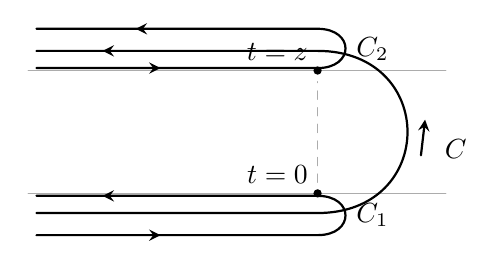
\begin{tikzpicture}[x=1.05cm,y=.78cm,>=stealth,line cap=round,line join=round]
  \draw[gray!65,thin] (-3.5,1)--(1.55,1);
  \draw[gray!65,thin] (-3.5,-1)--(1.55,-1);
  \fill (0,1) circle (1.5pt) node[above left] {$t=z$};
  \fill (0,-1) circle (1.5pt) node[above left] {$t=0$};
  \draw[gray!65,dashed,thin] (0,-.82)--(0,.82);
  \draw[thick] (-3.4,1.32)--(0,1.32)
    .. controls (1.45,1.32) and (1.45,-1.32) .. (0,-1.32)
    --(-3.4,-1.32);
  \draw[->,thick] (1.25,-.38)--(1.30,.20);
  \draw[->,thick] (-1.9,1.32)--(-2.6,1.32);
  \draw[->,thick] (-1.5,1.68)--(-2.2,1.68);
  \draw[thick] (-3.4,1.68)--(0,1.68)
    .. controls (.45,1.68) and (.45,1.04) .. (0,1.04)
    --(-3.4,1.04);
  \draw[->,thick] (-2.6,1.04)--(-1.9,1.04);
  \draw[thick] (-3.4,-1.04)--(0,-1.04)
    .. controls (.45,-1.04) and (.45,-1.68) .. (0,-1.68)
    --(-3.4,-1.68);
  \draw[->,thick] (-1.9,-1.04)--(-2.6,-1.04);
  \draw[->,thick] (-2.6,-1.68)--(-1.9,-1.68);
  \node[right] at (1.42,-.28) {$C$};
  \node[right] at (.35,1.35) {$C_2$};
  \node[right] at (.35,-1.35) {$C_1$};
\end{tikzpicture}
\caption{ }\label{fig:56}
\end{figure}

\SourcePage{786}{789}
At $z=0$ the two singular points of the integrand coalesce. A familiar formula
from the theory of the $\Gamma$-function gives
\begin{equation}
 \frac1{2\pi i}\int_C e^tt^{-\gamma}\,dt=\frac1{\Gamma(\gamma)}.
 \tag{d.7}
\end{equation}
Since $F(\alpha,\gamma,0)=1$, it is evident that
\begin{equation}
 F(\alpha,\gamma,z)=\frac{\Gamma(\gamma)}{2\pi i}
 \int_Ce^t(t-z)^{-\alpha}t^{\alpha-\gamma}\,dt.
 \tag{d.8}
\end{equation}

The integrand in (d.5) has singular points at $t=0$ and $t=1$. If
$\operatorname{Re}(\gamma-\alpha)>0$ and $\gamma$ is not a positive integer,
the path of integration may be taken to be a contour $C'$ that leaves $t=1$,
encircles $t=0$ in the positive sense, and returns to $t=1$ (Fig.~57). For
$\operatorname{Re}(\gamma-\alpha)>0$, traversal of this contour returns the
function $V(t)$ to its initial value, zero.\footnote{If $\gamma$ is a positive
integer, any contour encircling both $t=0$ and $t=1$ may be chosen as $C'$.}
The integral so defined is likewise nonsingular at $z=0$ and is related to
$F(\alpha,\gamma,z)$ by
\begin{equation}
 F(\alpha,\gamma,z)=-\frac1{2\pi i}
 \frac{\Gamma(1-\alpha)\Gamma(\gamma)}{\Gamma(\gamma-\alpha)}
 \oint_{C'}e^{tz}(-t)^{\alpha-1}(1-t)^{\gamma-\alpha-1}\,dt.
 \tag{d.9}
\end{equation}

\begin{figure}[ht]
\centering
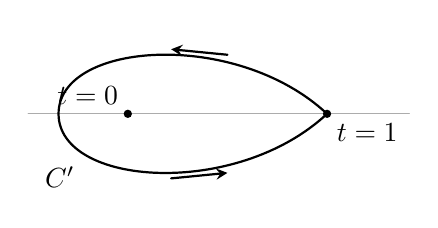
\begin{tikzpicture}[x=1.1cm,y=1cm,>=stealth,line cap=round,line join=round]
  \draw[gray!65,thin] (-2.2,0)--(2.2,0);
  \fill (-1.05,0) circle (1.5pt) node[above left] {$t=0$};
  \fill (1.25,0) circle (1.5pt) node[below right] {$t=1$};
  \draw[thick] (1.25,0) .. controls (.2,1.08) and (-1.85,.92) .. (-1.85,0)
    .. controls (-1.85,-.92) and (.2,-1.08) .. (1.25,0);
  \draw[->,thick] (.1,.75)--(-.55,.82);
  \draw[->,thick] (-.55,-.82)--(.1,-.75);
  \node[below left] at (-1.55,-.55) {$C'$};
\end{tikzpicture}
\caption{ }\label{fig:57}
\end{figure}

The following qualification concerning the integrals (d.8) and (d.9) is
necessary. For nonintegral $\alpha$ and $\gamma$, their integrands are
multiple-valued functions. At each point their values are understood to be
selected by requiring every complex quantity raised to a power to have the
argument of smallest absolute value.

We also note the useful relation
\begin{equation}
 F(\alpha,\gamma,z)=e^zF(\gamma-\alpha,\gamma,-z),
 \tag{d.10}
\end{equation}
which follows at once upon making the substitution $t\to t+z$ in (d.8).

It was already mentioned that when $\alpha=-n$, with $n$ a positive integer,
$F(\alpha,\gamma,z)$ reduces to a polynomial. A compact formula can be found
for these polynomials. Making the substitution $t\to1-(t/z)$ in (d.9) and
applying the Cauchy formula to

\SourcePage{787}{790}
the resulting integral, we find
\begin{equation}
 F(-n,\gamma,z)=\frac{z^{1-\gamma}e^z}
 {\gamma(\gamma+1)\cdots(\gamma+n-1)}
 \frac{d^n}{dz^n}\left(e^{-z}z^{\gamma+n-1}\right).
 \tag{d.11}
\end{equation}
If, in addition, $\gamma=m$, where $m$ is a positive integer, one also has
\begin{equation}
 F(-n,m,z)=\frac{(-1)^{m-1}e^zz^{1-m-n}}
 {m(m+1)\cdots(m+n-1)}
 \frac{d^{m+n-1}}{dz^{m+n-1}}\left(e^{-z}z^n\right).
 \tag{d.12}
\end{equation}
This formula results by applying the Cauchy formula to the integral obtained
from (d.8) through the substitution $t\to z-t$.

Up to a constant factor, the polynomials $F(-n,m,z)$ ($0\le m\le n$) are the
\emph{generalized Laguerre polynomials}:
\begin{equation}
 \begin{split}
 L_n^m(z)&=(-1)^m\frac{(n!)^2}{m!(n-m)!}
 F(-(n-m),m+1,z)\\
 &=\frac{n!}{(n-m)!}e^z\frac{d^m}{dz^m}
 \left(e^{-z}z^{n-m}\right)\\
 &=(-1)^m\frac{n!}{(n-m)!}e^zz^{-m}
 \frac{d^{n-m}}{dz^{n-m}}\left(e^{-z}z^n\right).
 \end{split}
 \tag{d.13}
\end{equation}
For $m=0$, the polynomials $L_n^m$ are denoted by $L_n(z)$ and are called
simply the \emph{Laguerre polynomials}; according to (d.13),
\[
 L_n(z)=e^z\frac{d^n}{dz^n}\left(e^{-z}z^n\right).
\]

The integral representation (d.8) is useful in finding the asymptotic
expansion of the confluent hypergeometric function for large $z$. Deform the
contour until it becomes two contours $C_1$ and $C_2$ (see Fig.~56), which
encircle $t=0$ and $t=z$, respectively; the lower branch of $C_2$ and the
upper branch of $C_1$ are to be regarded as joining at infinity. To obtain an
expansion in inverse powers of $z$, take the factor $(-z)^{-\alpha}$ outside
the integrand. In the integral along $C_2$, make the substitution $t\to t+z$;
this changes $C_2$ into $C_1$. Formula (d.8) is thereby written as
\begin{equation}
 \begin{split}
 F(\alpha,\gamma,z)
 &=\frac{\Gamma(\gamma)}{\Gamma(\gamma-\alpha)}
 (-z)^{-\alpha}G(\alpha,\alpha-\gamma+1,-z)\\
 &\hspace{1.5em}+\frac{\Gamma(\gamma)}{\Gamma(\alpha)}
 e^zz^{\alpha-\gamma}G(\gamma-\alpha,1-\alpha,z),
 \end{split}
 \tag{d.14}
\end{equation}

\SourcePage{788}{791}
where
\begin{equation}
 G(\alpha,\beta,z)=\frac{\Gamma(1-\beta)}{2\pi i}
 \int_{C_1}\left(1+\frac tz\right)^{-\alpha}t^{\beta-1}e^t\,dt.
 \tag{d.15}
\end{equation}
When powers are taken in (d.14), $-z$ and $z$ must be assigned the arguments
of smallest absolute value. Finally, expand $(1+t/z)^{-\alpha}$ in powers of
$t/z$ in the integrand and use (d.7). The resulting asymptotic series for
$G(\alpha,\beta,z)$ is
\begin{equation}
 G(\alpha,\beta,z)=1+\frac{\alpha\beta}{1!z}
 +\frac{\alpha(\alpha+1)\beta(\beta+1)}{2!z^2}+\ldots
 \tag{d.16}
\end{equation}
Equations (d.14) and (d.16) specify the asymptotic expansion of
$F(\alpha,\gamma,z)$.

For positive integral $\gamma$, the second term in the general solution (d.4)
of equation (d.2) either coincides with the first (when $\gamma=1$) or becomes
altogether meaningless (when $\gamma>1$). In this case, the two terms in
(d.14) may be chosen as a pair of linearly independent solutions, that is, the
integrals (d.8) taken along $C_1$ and $C_2$. (These contours, like $C$, satisfy
the required conditions, so their integrals are also solutions of (d.2).)
Their asymptotic forms have already been given; it remains to determine their
expansions in ascending powers of $z$. For this purpose, begin with (d.14) and
the analogous equality for the function
$z^{1-\gamma}F(\alpha-\gamma+1,2-\gamma,z)$. From these two equalities, express
$G(\alpha,\alpha-\gamma+1,-z)$ in terms of $F(\alpha,\gamma,z)$ and
$F(\alpha-\gamma+1,2-\gamma,z)$, then put $\gamma=p+\varepsilon$ ($p$ being a
positive integer) and take the limit $\varepsilon\to0$, resolving the
indeterminate forms by l'Hopital's rule. A fairly lengthy calculation gives
the expansion
\begin{equation}
 \small
 \begin{split}
 G(\alpha,\alpha-p+1,-z)
 &=-\frac{\sin\pi\alpha\,\Gamma(p-\alpha)}{\pi\Gamma(p)}z^\alpha
 \Biggl\{\ln z\,F(\alpha,p,z)\\
 &\hspace{1.5em}+\sum_{s=0}^{\infty}
 \frac{\Gamma(p)\Gamma(\alpha+s)
 [\psi(\alpha+s)-\psi(p+s)-\psi(s+1)]}
 {\Gamma(\alpha)\Gamma(s+p)\Gamma(s+1)}z^s\\
 &\hspace{1.5em}+\sum_{s=1}^{p-1}(-1)^{s+1}
 \frac{\Gamma(s)\Gamma(\alpha-s)\Gamma(p)}
 {\Gamma(\alpha)\Gamma(p-s)}z^{-s}\Biggr\},
 \end{split}
 \tag{d.17}
\end{equation}
where $\psi$ denotes the logarithmic derivative of the $\Gamma$-function:
$\psi(\alpha)=\Gamma'(\alpha)/\Gamma(\alpha)$.
